\documentclass[12pt]{article}

\usepackage[a4paper,margin=1in]{geometry}
\usepackage{setspace}
\usepackage{longtable}
\usepackage{array}
\usepackage{titlesec}
\usepackage{enumitem}
\usepackage{graphicx}
\usepackage{booktabs}
\usepackage{float}
\usepackage[hidelinks]{hyperref}

\pdfsuppresswarningpagegroup=1
\setstretch{1.12}
\setlength{\emergencystretch}{3em}
\setlist[itemize]{noitemsep, topsep=0.35em}
\setlist[enumerate]{noitemsep, topsep=0.35em}
\renewcommand{\arraystretch}{1.18}
\newcolumntype{L}[1]{>{\raggedright\arraybackslash}p{#1}}

\begin{document}

\hypersetup{pageanchor=false}
\begin{titlepage}
\centering
\vspace*{1.2cm}
{\Large\textbf{Software Requirements Specification}\par}
\vspace{1.2cm}
{\huge\textbf{SchEDU}\par}
\vspace{0.45cm}
{\large\textbf{Adaptive Academic Pacing Using Deterministic Constraint-Based Greedy Scheduling and Heuristic Rebalancing}\par}
\vfill
{\large\textbf{Prepared by}\par}
\vspace{0.35cm}
{\large Aundreka Clarinze Perez\par}
{\large Marjinel Abante\par}
{\large Leo Franklin Borromeo\par}
\vfill
{\large College of Information Technology and Computer Science\par}
{\large Lyceum of the Philippines University -- Cavite\par}
\vspace{0.35cm}
{\large Software Engineering 2\par}
\vfill
{\large May 14, 2026\par}
\end{titlepage}

\hypersetup{pageanchor=true}
\pagenumbering{roman}
\tableofcontents
\newpage

\section*{Document Control}
\addcontentsline{toc}{section}{Document Control}

\begin{longtable}{|L{3.5cm}|L{10.2cm}|}
\hline
\textbf{Document Title} & Software Requirements Specification for SchEDU \\
\hline
\textbf{System Name} & SchEDU: Adaptive Academic Pacing Using Deterministic Constraint-Based Greedy Scheduling and Heuristic Rebalancing \\
\hline
\textbf{Prepared By} & Aundreka Clarinze Perez, Marjinel Abante, and Leo Franklin Borromeo \\
\hline
\textbf{Institution} & College of Information Technology and Computer Science, Lyceum of the Philippines University -- Cavite \\
\hline
\textbf{Course Context} & Software Engineering 2 \\
\hline
\textbf{Version} & Rev. 2 \\
\hline
\textbf{Date} & May 14, 2026 \\
\hline
\textbf{Implementation Status} & Defense prototype with implemented mobile workflows, Supabase-backed persistence, repository-local scheduling logic, and auxiliary document services. \\
\hline
\end{longtable}

\subsection*{Revision History}
\addcontentsline{toc}{subsection}{Revision History}

\begin{longtable}{|L{2.5cm}|L{2.8cm}|L{8.4cm}|}
\hline
\textbf{Revision} & \textbf{Date} & \textbf{Description} \\
\hline
Rev. 1 & May 14, 2026 & Initial repository-aligned SRS covering implemented SchEDU features and scheduler behavior. \\
\hline
Rev. 2 & May 14, 2026 & Added formal title page, separated table of contents, strengthened defense-ready implementation scope, clarified live-demo assumptions, added acceptance criteria and traceability evidence, and tightened requirement wording. \\
\hline
\end{longtable}

\newpage
\pagenumbering{arabic}

\section{Introduction}

\subsection{Purpose}

This Software Requirements Specification (SRS) defines the functional,
non-functional, interface, data, validation, and demonstration requirements of
SchEDU. The document is intended to serve as the shared specification for
implementation, evaluation, testing, documentation, and academic defense of the
current system. It describes the implemented defense prototype rather than an
abstract future proposal, while still identifying boundaries that are not claimed
by the current repository.

\subsection{Product Scope}

SchEDU is a mobile academic planning system for teachers. It consolidates
curriculum organization, lesson planning, deterministic schedule generation,
calendar maintenance, curriculum text extraction, and AI-assisted activity
generation within a single application. The system is designed around
teacher-level instructional planning rather than institution-wide room
allocation, student enrollment management, or global campus timetabling.

For defense purposes, SchEDU is treated as a full implemented system that can be
demonstrated live through authenticated mobile workflows. A successful demo
should show a teacher moving from account access and academic setup to subject
content, lesson-plan generation, calendar inspection, disruption handling, and
document-support workflows using repository-backed code and Supabase-backed data.

The current system supports the following major capabilities:
\begin{itemize}
\item authenticated user access with profile and theme management;
\item institution, section, and subject management;
\item structured storage of units, chapters, lessons, and lesson-plan scope;
\item deterministic rule-based schedule generation, compression, and rebalance;
\item monthly and daily calendar views with block-level maintenance actions; and
\item document support workflows for curriculum extraction and activity generation.
\end{itemize}

\subsection{Intended Audience}

This document is intended for the following stakeholders:
\begin{itemize}
\item project proponents and panel members who need a precise system definition;
\item developers implementing or extending the application;
\item testers validating requirements against system behavior;
\item teachers and pilot users reviewing supported workflows; and
\item administrators evaluating operational and reporting capabilities.
\end{itemize}

\subsection{Definitions and Acronyms}

\begin{longtable}{|L{3.5cm}|L{10.2cm}|}
\hline
\textbf{Term} & \textbf{Definition} \\
\hline
SRS & Software Requirements Specification. \\
\hline
OAuth & Third-party authentication flow such as Google, Apple, or Facebook sign-in. \\
\hline
OCR & Optical Character Recognition used to extract text from images. \\
\hline
RLS & Row-Level Security used by Supabase/PostgreSQL to restrict data access. \\
\hline
Lesson Plan & A teacher-owned planning record that binds a subject, section, date range, and selected content to generated schedule state. \\
\hline
Slot & A schedulable class meeting occurrence derived from recurring meeting patterns and date ranges. \\
\hline
Block & A scheduled instructional or assessment unit such as a lesson, written work, performance task, exam, or buffer. \\
\hline
Blackout & A date or slot made unavailable by events, delays, suspension, leave, or related constraints. \\
\hline
PT & Performance Task. \\
\hline
WW & Written Work. \\
\hline
\end{longtable}

\subsection{Document Overview}

Section 2 describes the product context, actors, operating environment,
constraints, and live-demo assumptions. Section 3 defines the external
interfaces. Section 4 defines the core data requirements. Section 5 lists the
functional requirements by feature area. Section 6 defines non-functional
requirements. Section 7 defines acceptance criteria and traceability evidence.
Section 8 records the current system boundaries to prevent overclaiming
unsupported behavior.

\section{Overall Description}

\subsection{Product Perspective}

SchEDU is a client-server mobile application built with React Native and Expo
Router on the client side and Supabase services on the backend. The client
contains the primary planning workflows, while the backend manages user access,
structured academic records, stored files, and server-side utility functions.

\begin{figure}[H]
\centering
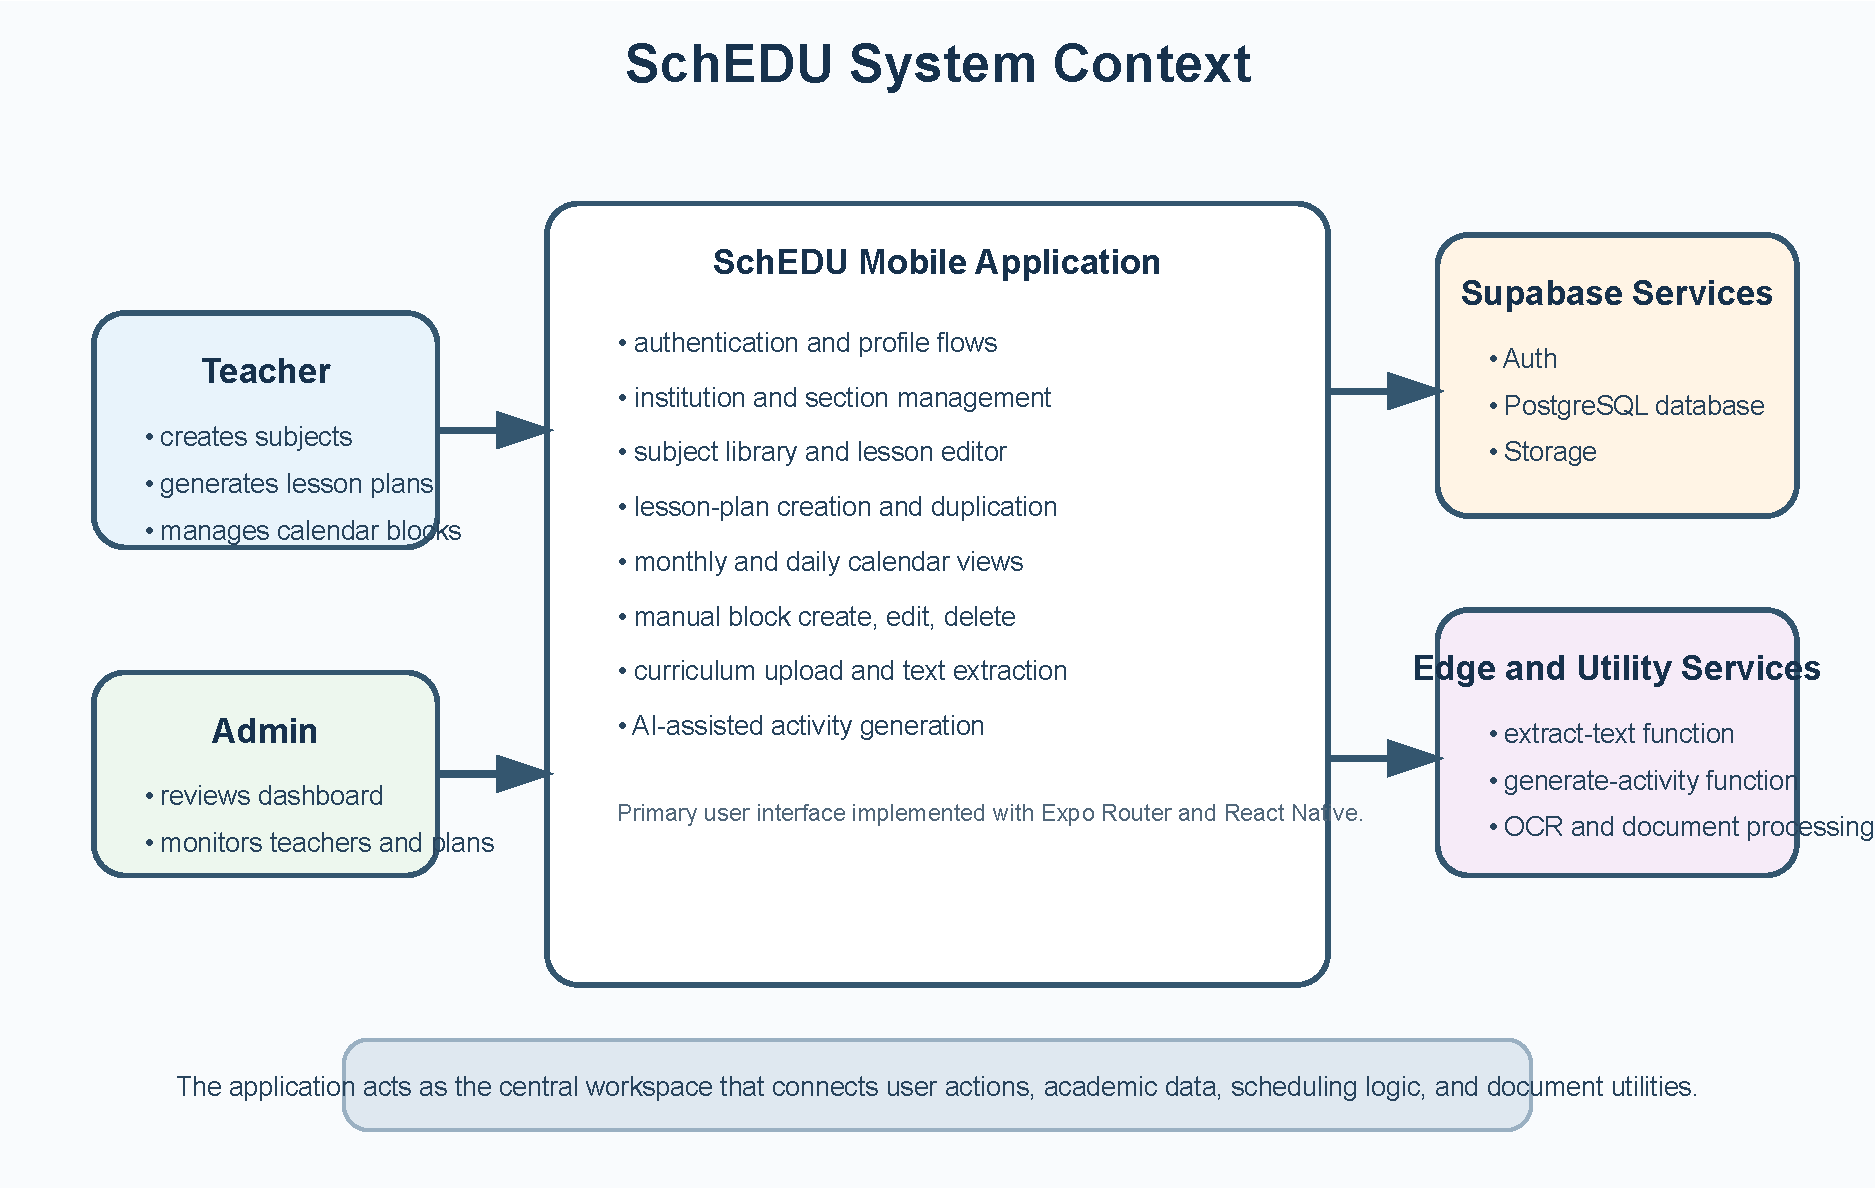
\includegraphics[height=0.28\textheight,keepaspectratio]{figures/system-context.pdf}
\caption{SchEDU system context}
\label{fig:system-context}
\end{figure}

As shown in Figure~\ref{fig:system-context}, teachers and administrators use the
same application context but interact with different feature subsets. The mobile
application acts as the central workspace that coordinates persistent academic
data, scheduling logic, and supporting utility services.

\subsection{Product Functions}

At a high level, the system provides the following functions:
\begin{itemize}
\item authenticate users and maintain profile, theme, and session state;
\item manage institutions, sections, subjects, units, chapters, and lessons;
\item create lesson plans using selected content, date ranges, and meeting
patterns;
\item generate schedule slots and blocks using a deterministic
constraint-based greedy scheduler;
\item display lesson-plan outputs in plan, monthly calendar, and daily agenda
views;
\item allow block-level maintenance such as create, edit, delete, suspend, and
refresh actions;
\item extract text from uploaded curriculum documents; and
\item generate and export classroom activity drafts in PDF and DOCX formats.
\end{itemize}

\subsection{Scheduling Methodology}

The scheduler is implemented as a deterministic constructive pipeline rather than
as a global search or metaheuristic procedure. A single run consumes the
lesson-plan record, recurring meeting patterns, selected lesson scope, stored
activity requirements, academic-term rules, blackout events, delay records, and
any existing slot or block state that must be preserved. The scheduler emits
runtime slots, runtime blocks, per-term schedule-plan metadata, ordered slot
output, warnings, and summary metrics.

The methodology proceeds in the following stages:
\begin{enumerate}
\item \textbf{Slot normalization and expansion.} Meeting patterns are normalized
by weekday and time, assigned stable slot numbers and series keys, validated so
that overlapping same-day instances are rejected, and expanded across the
lesson-plan date range into dated runtime slots.
\item \textbf{Blackout mapping and slot-state merge.} School calendar events and
teacher delays are mapped onto slot dates as blackout information. Existing slot
rows may be merged into generated slots so that persistent identifiers and manual
lock state can survive regeneration where applicable.
\item \textbf{Term decomposition and block derivation.} Usable slots are grouped
into academic terms ending on configured exam dates. Lessons, written work, and
performance-task counts are distributed across terms by deterministic equal
baseline allocation with earlier-term remainder priority, quiz blocks are
derived from lesson dependencies, and each term receives an exam block and its
exam-slot anchor. If no normal class slot exists on the exam date, a synthetic
exam slot is created for that term.
\item \textbf{Constraint-based greedy placement.} The scheduler reserves exam
slots first, then greedily assigns lesson blocks to the next usable chronological
content slot. Due quizzes are released when all prerequisite lessons have been
placed, while written work and performance tasks are inserted according to
computed term intervals. Placement is deterministic because the next feasible
slot and the next due block are always selected by fixed ordering rules rather
than by randomized search.
\item \textbf{Heuristic compression, ordering, and rebalance.} When usable slot
capacity is lower than the number of remaining content blocks, assessments may be
compressed onto compatible lesson slots according to bounded heuristics.
Non-quiz written work prefers a lesson slot already in use, while performance
tasks first prefer a lesson slot that does not already contain written work.
After placement, within-slot order is normalized for display stability. When
availability changes later, non-pinned blocks are released and re-flowed while
teacher-locked blocks, exam blocks, and protected buffers remain preserved where
possible.
\end{enumerate}

The methodology depends on one important implementation invariant: teacher
actions that must survive future rebalancing are represented as locked schedule
state. A manually pinned block that later becomes infeasible is surfaced as a
visible conflict for re-pinning rather than being silently relocated by the
scheduler.

\subsection{Live Demonstration Profile}

The system is expected to support a live defense demonstration using a configured
Expo/React Native build and a reachable Supabase project. The demonstration
should be prepared with sample academic data so that reviewers can observe the
implemented end-to-end behavior without waiting for manual data entry for every
record.

\begin{longtable}{|L{3.1cm}|L{5.3cm}|L{5.0cm}|}
\hline
\textbf{Demo Area} & \textbf{Expected Demonstration} & \textbf{Evidence of Completion} \\
\hline
Authentication and profile & Sign in, load the authenticated user context, and open profile or settings screens. & Protected routes load only after authentication and user metadata is displayed. \\
\hline
Academic setup & Open institution, section, subject, chapter, and lesson workflows. & Teacher-owned academic records appear in library and planning screens. \\
\hline
Lesson-plan generation & Select a subject, section, date range, meeting pattern, term dates, and lesson scope, then generate the plan. & Plan, slots, selected content, and blocks are persisted and visible in plan/calendar views. \\
\hline
Calendar maintenance & Open monthly and daily views, inspect blocks, create or edit a block, and suspend or restore a teaching day. & Calendar refreshes, blocks remain ordered, and schedule maintenance actions preserve data. \\
\hline
Rebalance and conflict handling & Trigger a blackout or suspension affecting a plan with scheduled blocks. & Non-locked blocks re-flow, locked conflicts remain visible, and no scheduled block is silently discarded. \\
\hline
Document support & Upload a curriculum source or invoke activity generation for written work or performance tasks. & Extracted or generated text is returned in an editable form and can be exported where configured. \\
\hline
Administrative overview & Open admin dashboard screens using an authorized role. & Teacher, subject, lesson-plan, and activity summaries render from backend records. \\
\hline
\end{longtable}

\subsection{Operational Prerequisites for Defense}

The following conditions must be satisfied before a live demonstration:
\begin{itemize}
\item a local or device build must have the required Expo/React Native runtime available;
\item \texttt{EXPO\_PUBLIC\_SUPABASE\_URL} and \texttt{EXPO\_PUBLIC\_SUPABASE\_KEY} must point to a provisioned Supabase project;
\item the database schema and RLS policies in the repository setup scripts must be applied;
\item demo users, school records, sections, subjects, and lessons should be prepared in advance;
\item the \texttt{extract-text} and \texttt{generate-activity} Edge Functions must be deployed for utility demonstrations;
\item image OCR should be demonstrated in a development build, not Expo Go, because the native OCR dependency requires native binaries; and
\item backup screenshots or prepared data should be available in case external network or AI service availability affects utility workflows.
\end{itemize}

\subsection{User Classes and Characteristics}

\begin{longtable}{|L{2.7cm}|L{3.7cm}|L{1.9cm}|L{4.7cm}|}
\hline
\textbf{User Class} & \textbf{Description} & \textbf{Skill Level} & \textbf{Typical Responsibilities} \\
\hline
Teacher & Primary end user who manages instructional content and schedules. & Moderate & Create subjects, lessons, activities, lesson plans, and maintain calendar state. \\
\hline
Admin & Administrative user who monitors teacher, subject, and lesson-plan summaries. & Moderate & Review dashboard metrics, recent activity, teacher counts, and plan completion indicators. \\
\hline
Superadmin & Elevated administrative role represented in the data model. & High & Perform the responsibilities of an admin with higher institutional authority where configured. \\
\hline
\end{longtable}

\subsection{Operating Environment}

\begin{itemize}
\item \textbf{Client platform:} React Native application built with Expo Router.
\item \textbf{Primary targets:} Android and iOS mobile devices.
\item \textbf{Backend platform:} Supabase Auth, PostgreSQL, Storage, and Edge Functions.
\item \textbf{Development environment:} Node.js, TypeScript, Expo toolchain, ESLint, and Git-based version control.
\item \textbf{Document utilities:} PDF and DOCX generation libraries, file upload support, and OCR/document extraction services.
\item \textbf{Defense validation environment:} local repository execution for scheduler invariants, Expo linting, and PDF generation through the installed TeX toolchain.
\end{itemize}

\subsection{Design and Implementation Constraints}

\begin{itemize}
\item The system depends on valid Supabase environment variables and network connectivity.
\item Most application features require an authenticated session.
\item Image OCR depends on a native-capable development build and is not fully supported in Expo Go.
\item Access to stored files is constrained by authenticated ownership and bucket policies.
\item The scheduler is deterministic and rule-based; it is not a metaheuristic or search-optimization engine.
\item Teacher-initiated block placements that must survive future rebalance depend on locked schedule state being preserved in storage.
\item AI-assisted activity generation depends on configured backend function credentials and should be presented as teacher-editable draft generation rather than autonomous final assessment authoring.
\end{itemize}

\subsection{Assumptions and Dependencies}

\begin{itemize}
\item Teachers will define valid lesson-plan date ranges and recurring meeting patterns.
\item Institutions will maintain accurate subject, section, and lesson content data.
\item Curriculum extraction and activity generation depend on backend utilities and external processing services being available.
\item The mobile user has permission to access local files or photos when uploading curriculum or template assets.
\item The live defense environment will include prepared demo records so that schedule generation, rebalance, extraction, and activity-generation flows can be shown within the available presentation time.
\end{itemize}

\section{External Interface Requirements}

\subsection{User Interfaces}

The system is organized around authenticated mobile workflows. Major user-facing
modules are shown in Figure~\ref{fig:functional-overview}.

\begin{figure}[H]
\centering
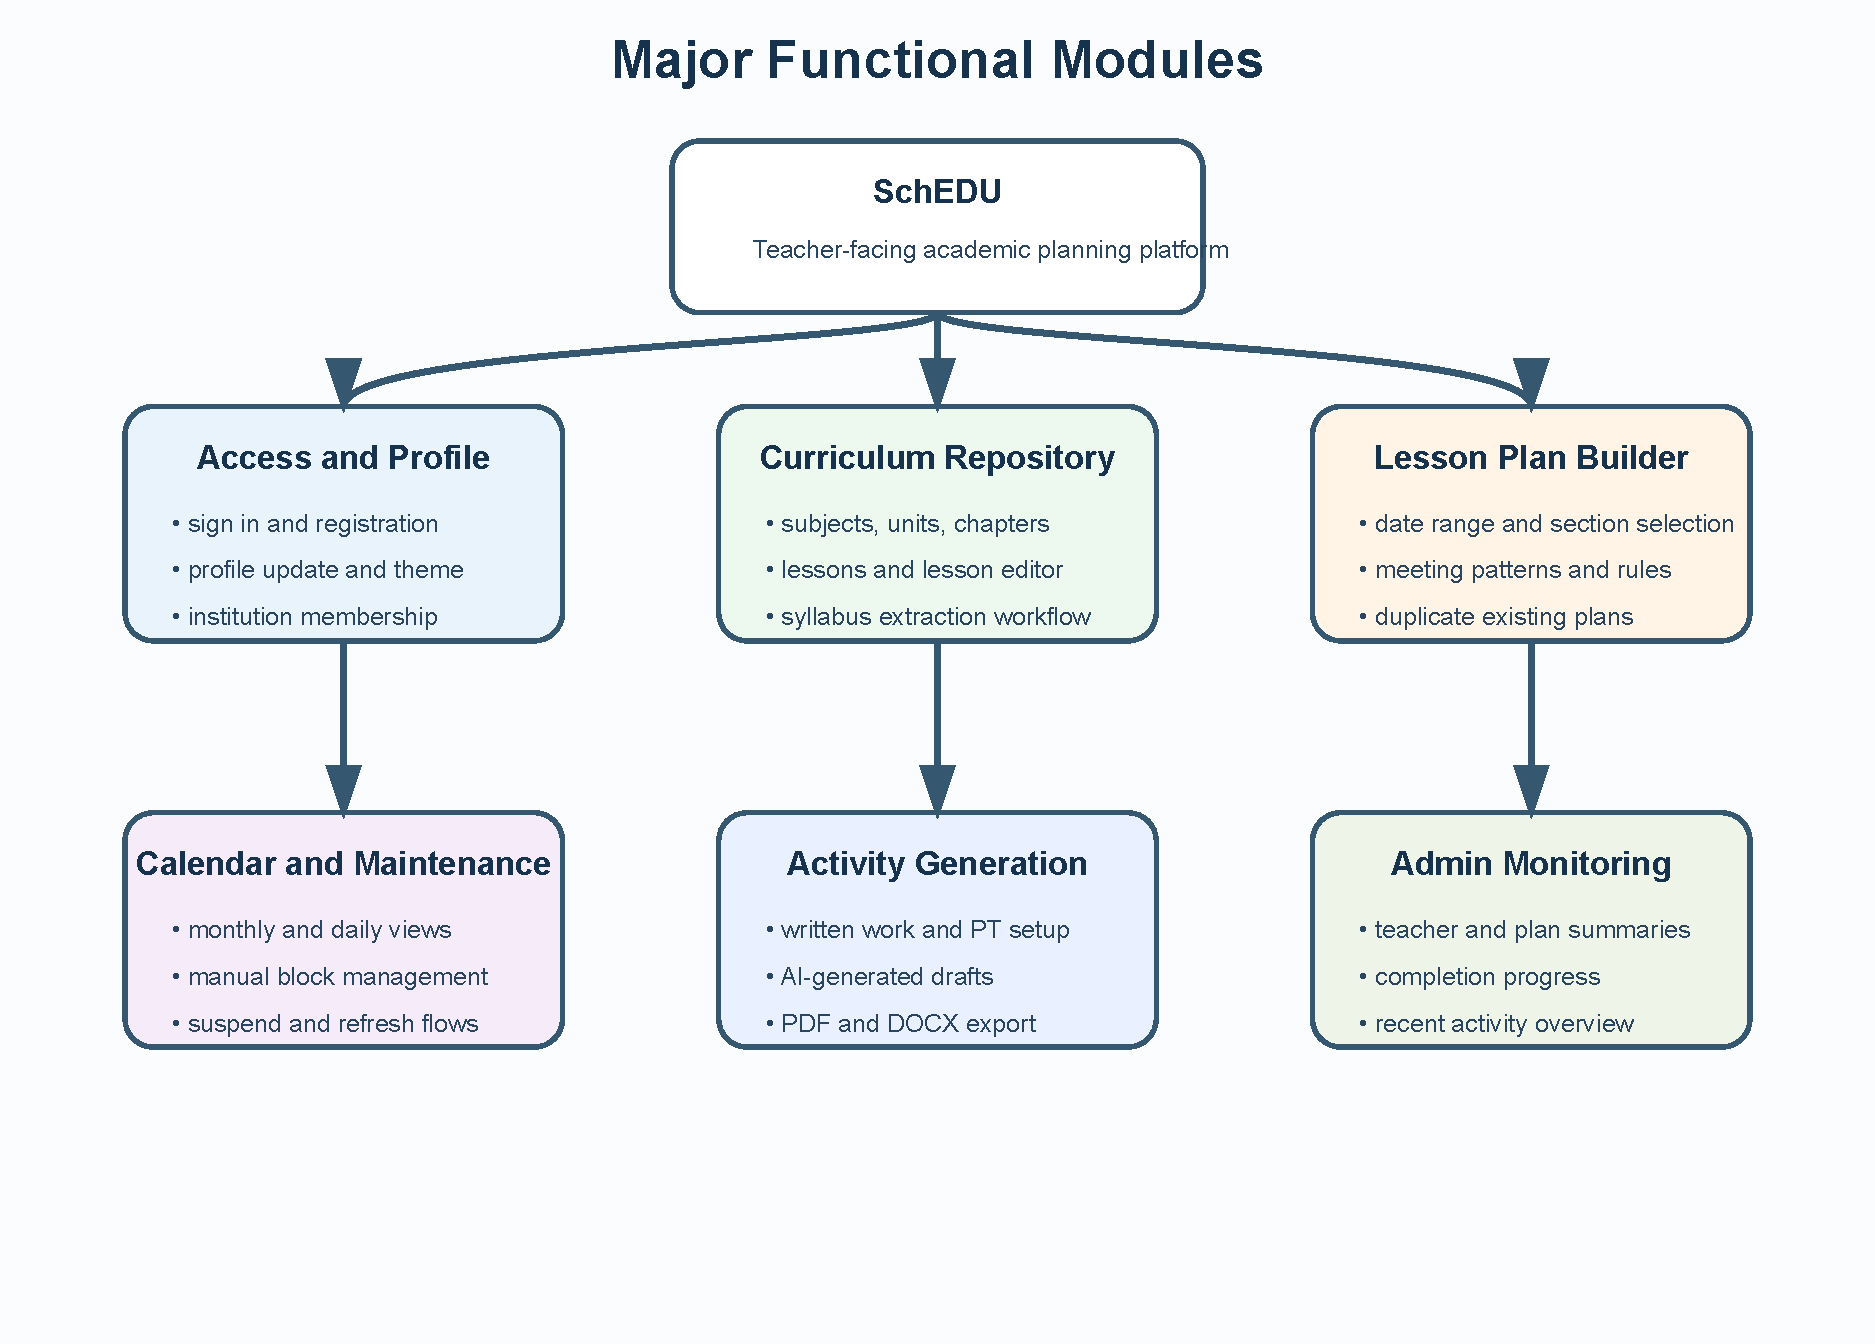
\includegraphics[height=0.28\textheight,keepaspectratio]{figures/functional-overview.pdf}
\caption{Major functional modules}
\label{fig:functional-overview}
\end{figure}

The major interface groups are:
\begin{itemize}
\item \textbf{Authentication interfaces:} sign-in, sign-up, forgot-password,
OAuth entry points, and password update screens.
\item \textbf{Profile interfaces:} profile summary, settings, appearance theme
selection, and institution detail screens.
\item \textbf{Library interfaces:} subject list, subject detail, lesson detail,
lesson editor, written-work detail, and performance-task detail screens.
\item \textbf{Planning interfaces:} lesson-plan creation, plan list, and plan
detail screens.
\item \textbf{Calendar interfaces:} monthly plan calendar, daily agenda, block
editor funnel, and suspension actions.
\item \textbf{Activity interfaces:} form-driven activity creation, AI generation,
preview, and export/share actions.
\item \textbf{Administrative interfaces:} dashboard summaries for teachers,
subjects, plans, and completion status.
\end{itemize}

\subsubsection{Representative UI Screens}

Figures~\ref{fig:ui-auth-screens} through~\ref{fig:ui-support-screens} show
representative screenshots from the current mobile application. These images
document the implemented interface style and the major workflow surfaces that
will be used in the live defense demonstration.

\begin{figure}[H]
\centering
\begin{minipage}{0.32\linewidth}
\centering
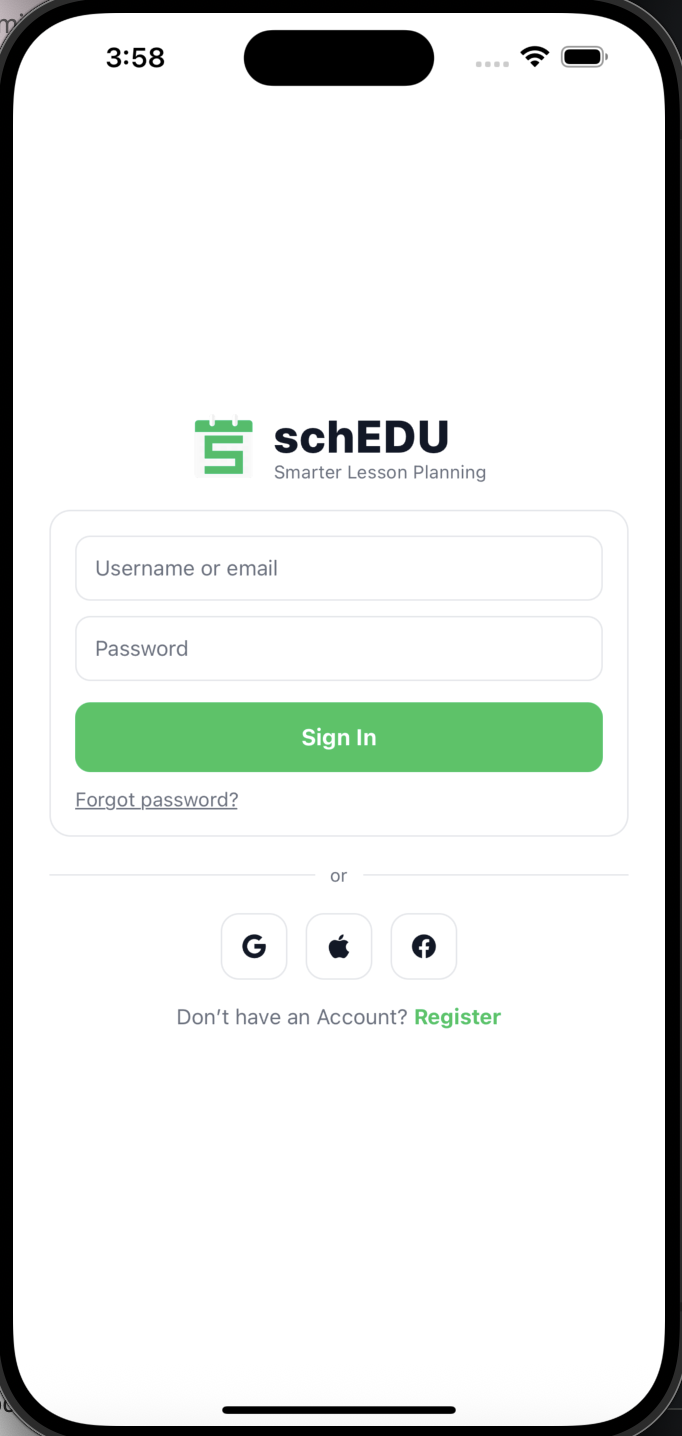
\includegraphics[height=0.32\textheight,keepaspectratio]{ui/login.png}\\
{\small Login}
\end{minipage}
\hfill
\begin{minipage}{0.32\linewidth}
\centering
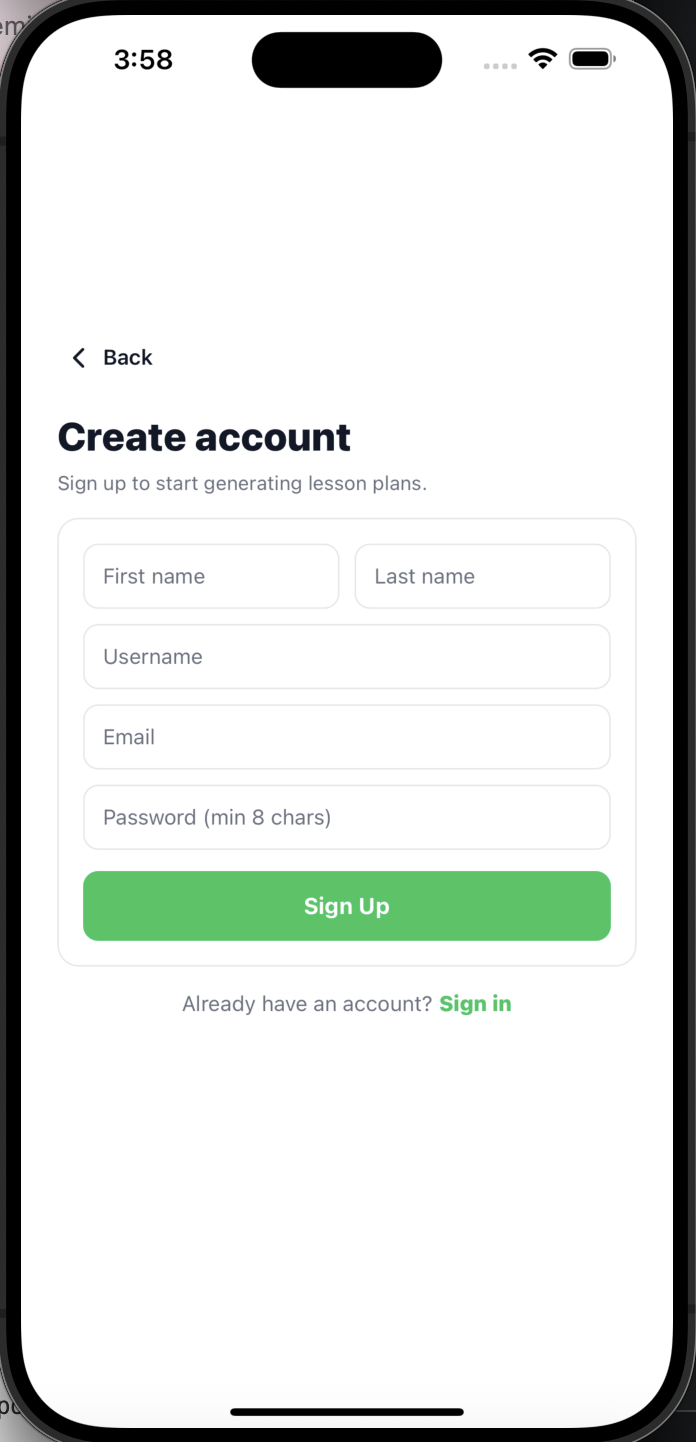
\includegraphics[height=0.32\textheight,keepaspectratio]{ui/register.png}\\
{\small Register}
\end{minipage}
\hfill
\begin{minipage}{0.32\linewidth}
\centering
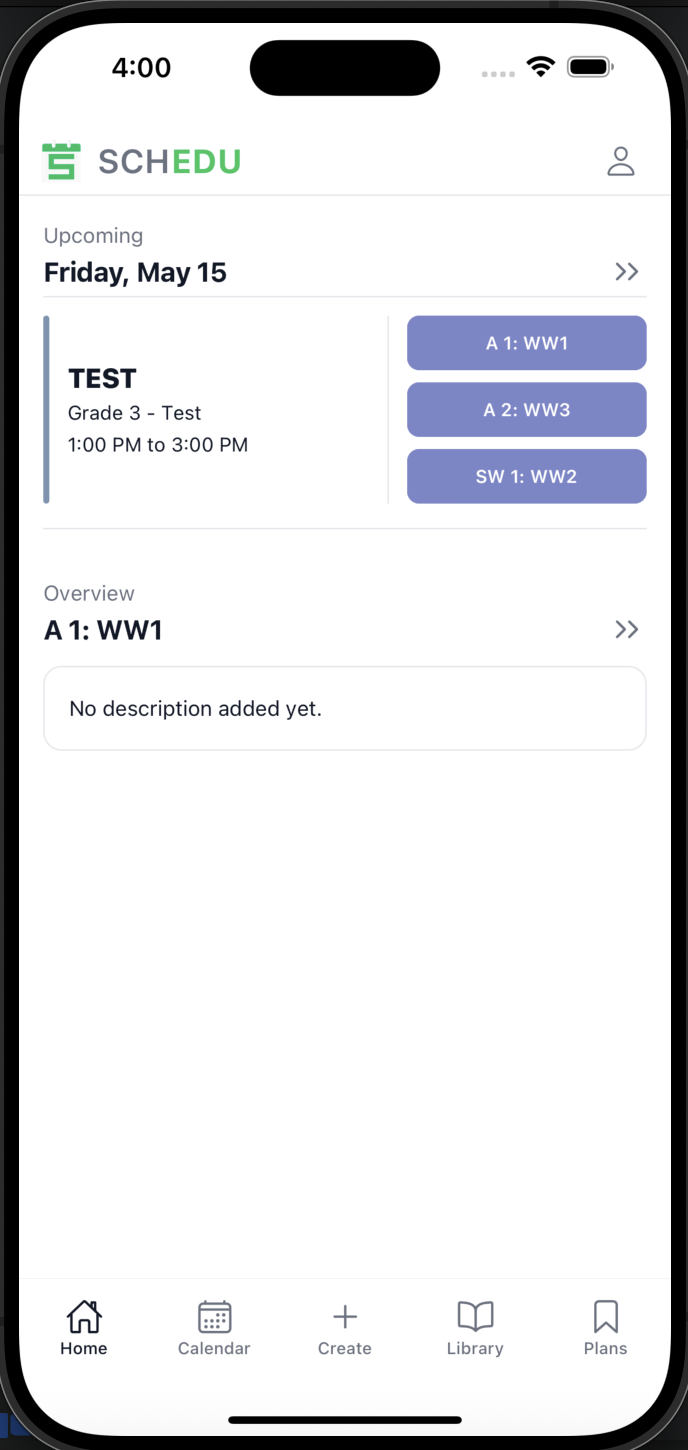
\includegraphics[height=0.32\textheight,keepaspectratio]{ui/dashboard.png}\\
{\small Dashboard}
\end{minipage}
\caption{Authentication and dashboard screens}
\label{fig:ui-auth-screens}
\end{figure}

\begin{figure}[H]
\centering
\begin{minipage}{0.32\linewidth}
\centering

\includegraphics[height=0.32\textheight,keepaspectratio]{ui/library.png}\\
{\small Library}
\end{minipage}
\hfill
\begin{minipage}{0.32\linewidth}
\centering
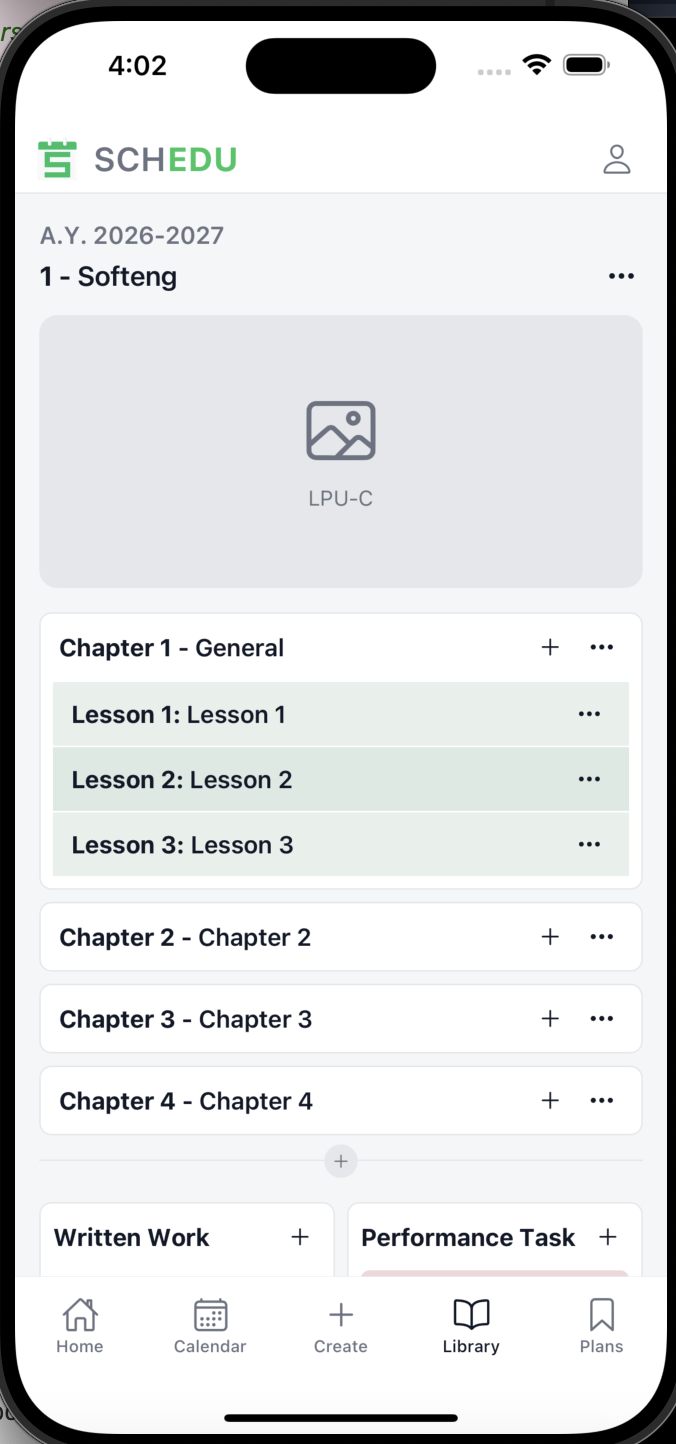
\includegraphics[height=0.32\textheight,keepaspectratio]{ui/subject.png}\\
{\small Subject Detail}
\end{minipage}
\hfill
\begin{minipage}{0.32\linewidth}
\centering
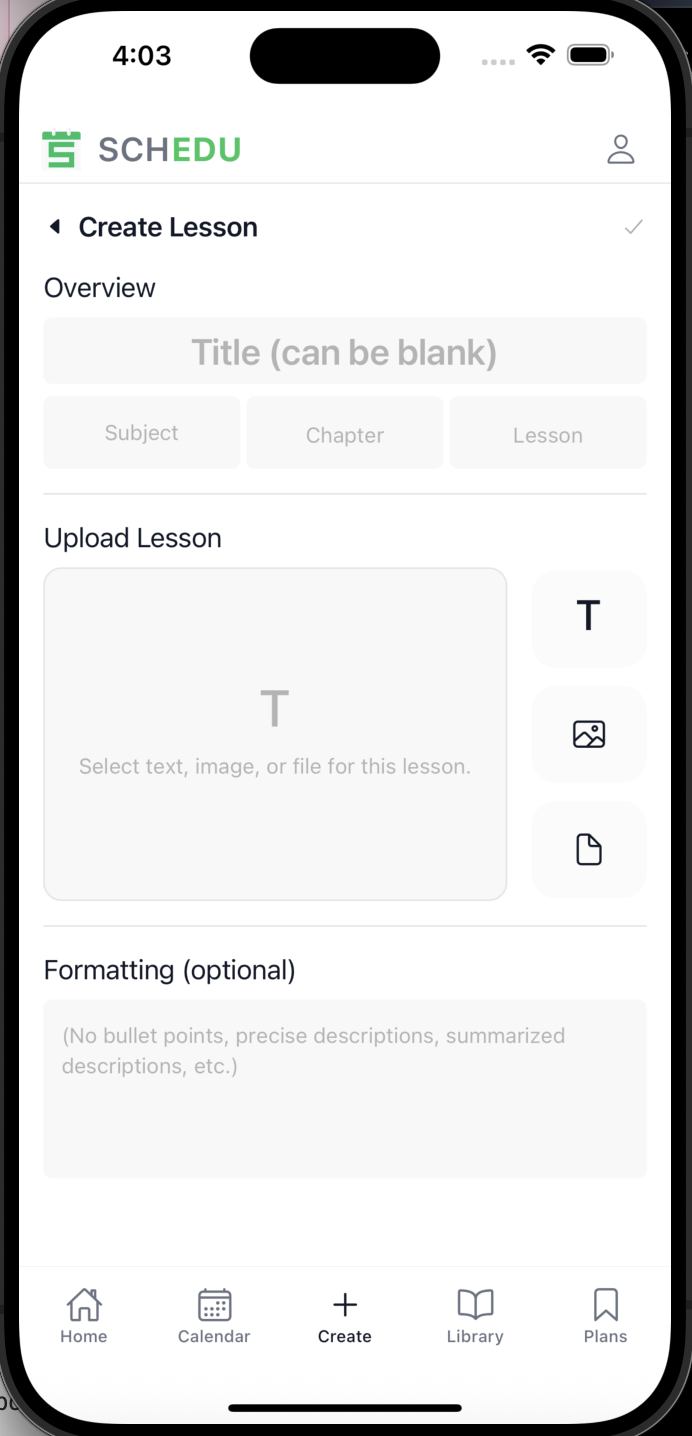
\includegraphics[height=0.32\textheight,keepaspectratio]{ui/lesson.png}\\
{\small Lesson Detail}
\end{minipage}
\caption{Curriculum library and lesson-content screens}
\label{fig:ui-library-screens}
\end{figure}

\begin{figure}[H]
\centering
\begin{minipage}{0.32\linewidth}
\centering
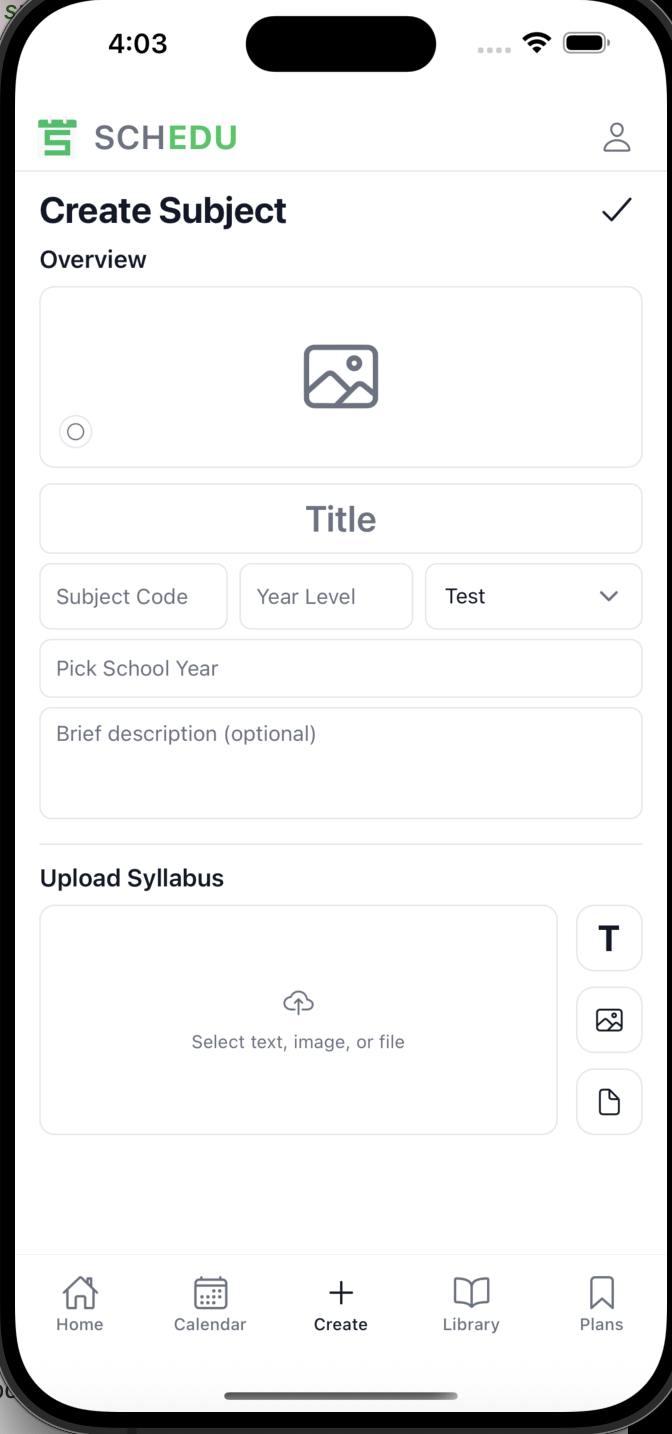
\includegraphics[height=0.32\textheight,keepaspectratio]{ui/createsubj.png}\\
{\small Create Subject}
\end{minipage}
\hfill
\begin{minipage}{0.32\linewidth}
\centering

\includegraphics[height=0.32\textheight,keepaspectratio]{ui/lessonplan.png}\\
{\small Create Lesson Plan}
\end{minipage}
\hfill
\begin{minipage}{0.32\linewidth}
\centering

\includegraphics[height=0.32\textheight,keepaspectratio]{ui/calendar.png}\\
{\small Calendar}
\end{minipage}
\caption{Subject creation, lesson-plan creation, and calendar screens}
\label{fig:ui-planning-screens}
\end{figure}

\begin{figure}[H]
\centering
\begin{minipage}{0.32\linewidth}
\centering

\includegraphics[height=0.32\textheight,keepaspectratio]{ui/plans.png}\\
{\small Plans}
\end{minipage}
\hfill
\begin{minipage}{0.32\linewidth}
\centering
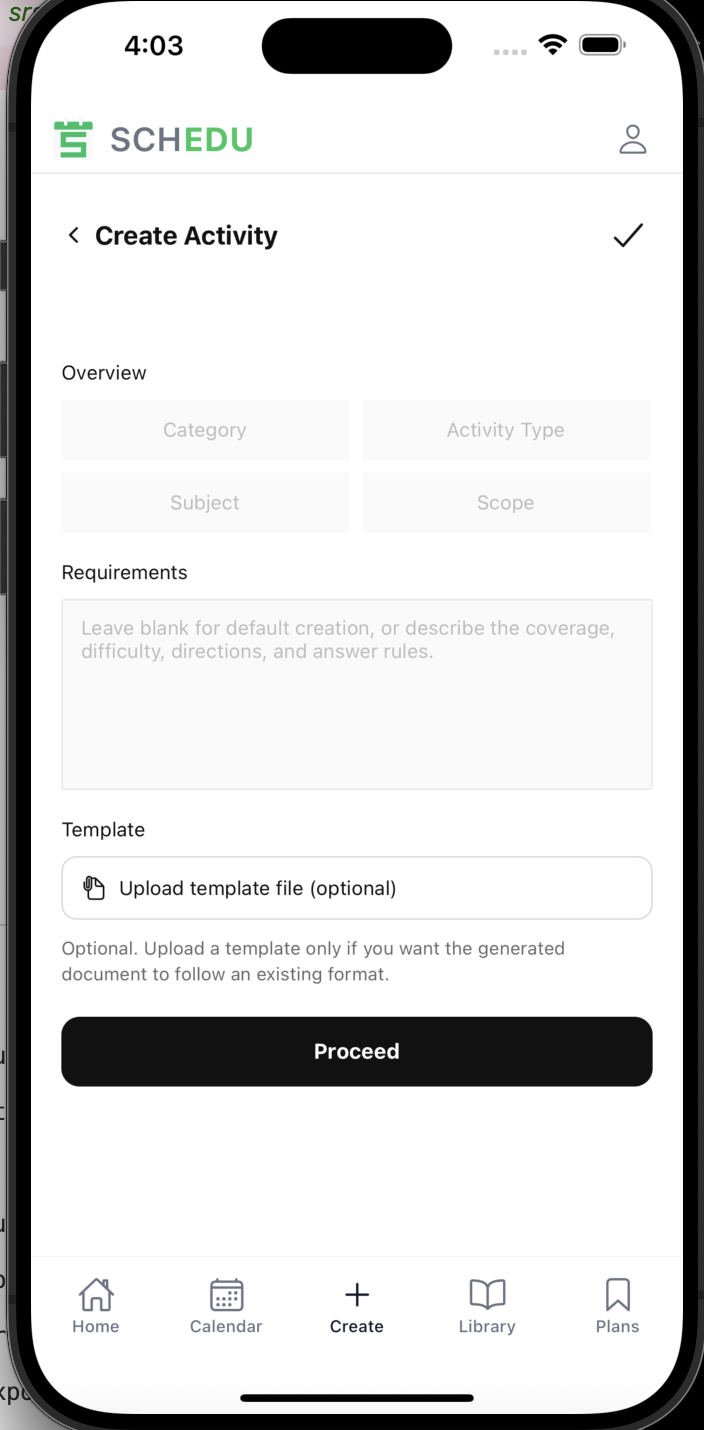
\includegraphics[height=0.32\textheight,keepaspectratio]{ui/activity.png}\\
{\small Activity Generation}
\end{minipage}
\hfill
\begin{minipage}{0.32\linewidth}
\centering
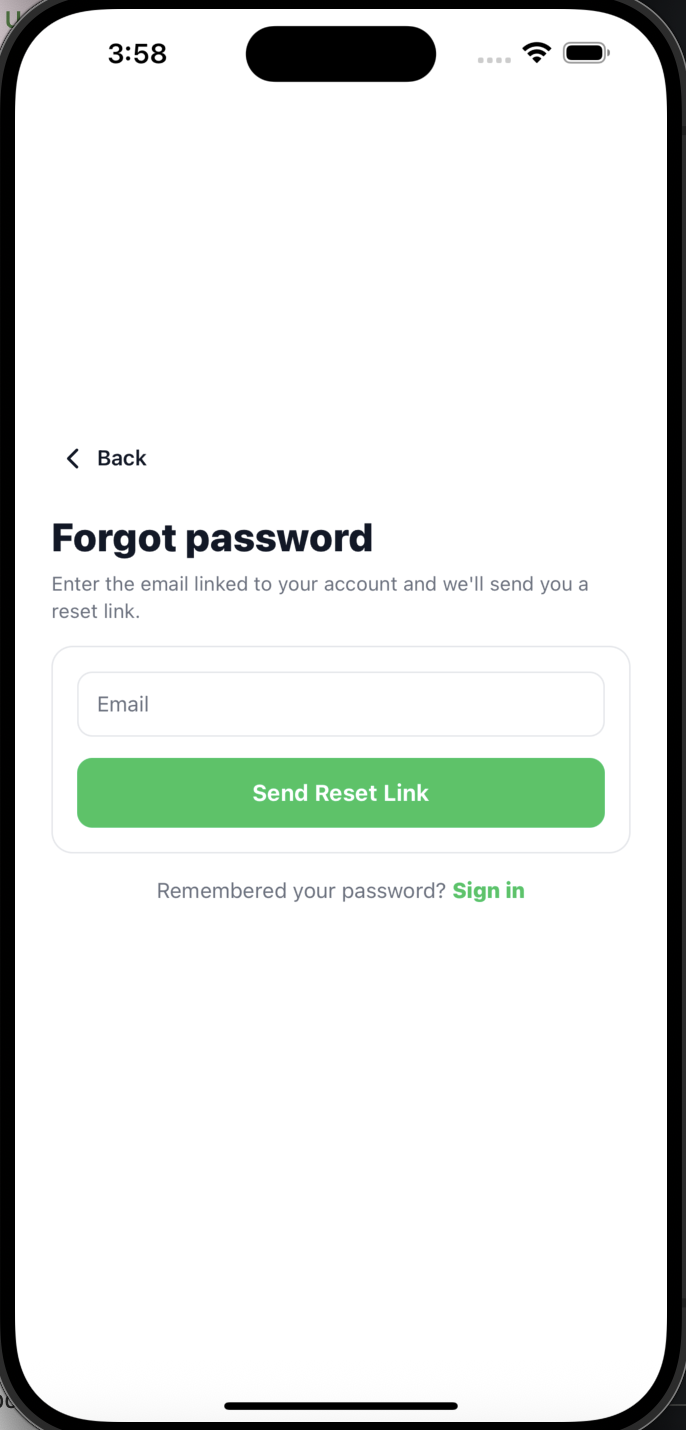
\includegraphics[height=0.32\textheight,keepaspectratio]{ui/resgister.png}\\
{\small Alternate Register View}
\end{minipage}
\caption{Plan management, activity-generation, and secondary account screen}
\label{fig:ui-support-screens}
\end{figure}

\subsection{Hardware Interfaces}

The application is intended for smartphones and tablets capable of running Expo
or native React Native builds. File upload features depend on local storage and,
for image-based flows, camera roll access or equivalent media permissions.

\subsection{Software Interfaces}

\begin{itemize}
\item \textbf{Supabase Auth:} user sign-in, sign-up, session persistence,
password reset, and OAuth integration.
\item \textbf{Supabase PostgreSQL:} structured storage for users, schools,
sections, subjects, units, chapters, lessons, lesson plans, slots, blocks,
calendar events, delays, and activities.
\item \textbf{Supabase Storage:} upload and retrieval of subject images, school
avatars, PDFs, and generated activity artifacts.
\item \textbf{Supabase Edge Functions:} \texttt{extract-text} and \texttt{generate-activity}.
\item \textbf{OCR library:} image text extraction in supported native builds.
\item \textbf{Document libraries:} PDF and DOCX generation for exported activity
files.
\end{itemize}

\subsection{Communication Interfaces}

The client communicates with Supabase services and Edge Functions over HTTPS. Data
exchange is primarily JSON-based for application records and multipart or binary
upload flows for files stored in the application bucket.

\section{Data Requirements}

\subsection{Core Data Entities}

\begin{longtable}{|L{3.2cm}|L{9.8cm}|}
\hline
\textbf{Entity} & \textbf{Description} \\
\hline
users & Stores teacher and administrative identity, role, and profile information. \\
\hline
schools & Stores institution records including school type, avatar data, and creator metadata. \\
\hline
sections & Stores academic sections associated with schools. \\
\hline
subjects & Stores teacher-owned subject records and syllabus-related metadata. \\
\hline
units, chapters, lessons & Store the curriculum hierarchy and lesson content used for planning. \\
\hline
lesson\_plans & Stores teacher lesson-plan context including subject, section, date range, and notes. \\
\hline
plan subject content & Stores the selected content scope used within a lesson plan. \\
\hline
slots & Stores generated or maintained schedule slots for a lesson plan. \\
\hline
blocks & Stores scheduled instructional and assessment units, including manual blocks. \\
\hline
school calendar events & Stores institution-level blackout events such as holidays, suspensions, and related blackout periods. \\
\hline
delays & Stores teacher- or plan-related delays and absence dates affecting planning. \\
\hline
activities & Stores AI-assisted written-work and performance-task drafts and associated artifacts. \\
\hline
\end{longtable}

\subsection{Data Integrity and Business Rules}

The system shall enforce the following data rules:
\begin{itemize}
\item lesson-plan end dates shall not be earlier than start dates;
\item slot end time shall be later than slot start time;
\item slot occurrences shall be unique per lesson plan, date, and slot number;
\item block category and subcategory pairings shall match supported instructional
types;
\item activities shall belong only to written-work or performance-task
categories;
\item sequence numbering for units, chapters, and lessons shall preserve
curriculum order within their parent scope;
\item teacher-pinned schedule edits that must survive regeneration or rebalance
shall be represented as locked slot or block state through the planner and
calendar workflows; and
\item user file access shall remain scoped to owned storage paths and
authenticated access policies.
\end{itemize}

\subsection{Data Lifecycle Requirements}

SchEDU data moves through a defined lifecycle during normal use:
\begin{enumerate}
\item the authenticated user creates or joins an institution context;
\item the user creates sections, subjects, and subject content;
\item a lesson plan binds the subject, section, date range, meeting pattern, and selected content scope;
\item the scheduler derives slots and blocks from the saved planning inputs;
\item calendar workflows read, edit, suspend, restore, or rebalance the persisted plan state; and
\item activity and extraction workflows store generated text, file paths, and supporting metadata under the authenticated user context.
\end{enumerate}

The system shall not treat generated schedule state as disposable UI-only data.
Slots, blocks, selected content scope, calendar events, delays, and activity
artifacts must remain inspectable through backend records so that a defense demo
can show continuity between data entry, generated output, and later maintenance.

\section{System Features and Functional Requirements}

\subsection{Authentication and Session Management}

\textbf{Description:} This feature set manages account access, password-based and
OAuth sign-in, recovery, and session routing.

\textbf{Priority: High}

\begin{longtable}{|L{2.3cm}|L{11.3cm}|}
\hline
\textbf{ID} & \textbf{Requirement} \\
\hline
FR-01 & The system shall allow a user to register an account using email and password credentials. \\
\hline
FR-02 & The system shall allow a user to sign in using email and password credentials. \\
\hline
FR-03 & The system shall support username-based sign-in by resolving the stored username to the associated email address. \\
\hline
FR-04 & The system shall support OAuth sign-in with the configured third-party providers. \\
\hline
FR-05 & The system shall provide a forgot-password flow for account recovery. \\
\hline
FR-06 & The system shall provide an update-password flow for authenticated password reset completion. \\
\hline
FR-07 & The system shall persist authenticated sessions and redirect signed-in users away from authentication screens. \\
\hline
FR-08 & The system shall redirect unauthenticated users away from protected application routes. \\
\hline
FR-09 & The system shall allow a signed-in user to terminate the current session by signing out. \\
\hline
\end{longtable}

\subsection{Profile, Theme, Institution, and Section Management}

\textbf{Description:} This feature set maintains the user's profile, appearance
settings, institution records, and sections.

\textbf{Priority: High}

\begin{longtable}{|L{2.3cm}|L{11.3cm}|}
\hline
\textbf{ID} & \textbf{Requirement} \\
\hline
FR-10 & The system shall allow a signed-in user to view stored profile details including first name, last name, username, and email. \\
\hline
FR-11 & The system shall allow a signed-in user to update profile details. \\
\hline
FR-12 & The system shall allow a signed-in user to change the application appearance theme among system, light, and dark modes. \\
\hline
FR-13 & The system shall display the institutions associated with the signed-in user. \\
\hline
FR-14 & The system shall allow a user to create a new institution record with a name, school type, and visual identity settings. \\
\hline
FR-15 & The system shall allow a user to upload and store an institution avatar image. \\
\hline
FR-16 & The system shall allow a user to update institution information, including name, type, avatar image, and avatar color. \\
\hline
FR-17 & The system shall allow a user to view all sections under a selected institution. \\
\hline
FR-18 & The system shall allow a user to create a new section for a selected institution. \\
\hline
FR-19 & The system shall allow a user to edit section details such as name and grade level. \\
\hline
FR-20 & The system shall allow a user to delete a section subject to backend constraints. \\
\hline
\end{longtable}

\subsection{Subject, Curriculum, and Lesson Management}

\textbf{Description:} This feature set stores academic content that becomes the
input to planning and scheduling workflows.

\textbf{Priority: High}

\begin{longtable}{|L{2.3cm}|L{11.3cm}|}
\hline
\textbf{ID} & \textbf{Requirement} \\
\hline
FR-21 & The system shall allow a user to create a subject under a selected institution. \\
\hline
FR-22 & The system shall allow a user to store subject metadata including code, title, year, academic year, description, and image. \\
\hline
FR-23 & The system shall allow a user to provide syllabus or curriculum input as direct text, uploaded image, or uploaded file. \\
\hline
FR-24 & The system shall upload syllabus-related assets to application storage under the authenticated user context. \\
\hline
FR-25 & The system shall allow a user to invoke curriculum text extraction for uploaded PDF or image assets. \\
\hline
FR-26 & The system shall allow a user to review and edit extracted or parsed curriculum text before saving subject content. \\
\hline
FR-27 & The system shall store curriculum hierarchy as units, chapters, and lessons. \\
\hline
FR-28 & The system shall allow a user to create lesson content manually without relying on imported curriculum text. \\
\hline
FR-29 & The system shall allow a user to store and edit lesson titles, content, learning objectives, and estimated lesson information. \\
\hline
FR-30 & The system shall display the authenticated user's subjects in a library view. \\
\hline
FR-31 & The system shall support searching and filtering the subject library by query, institution, and year where data is available. \\
\hline
FR-32 & The system shall allow a user to open a subject detail view showing related lesson and activity context. \\
\hline
FR-33 & The system shall provide lesson detail and lesson-editor screens for detailed lesson review and editing. \\
\hline
\end{longtable}

\subsection{Lesson Planning and Schedule Generation}

\textbf{Description:} This feature set creates lesson plans and translates stored
curriculum data into schedulable state.

\textbf{Priority: High}

\begin{figure}[H]
\centering
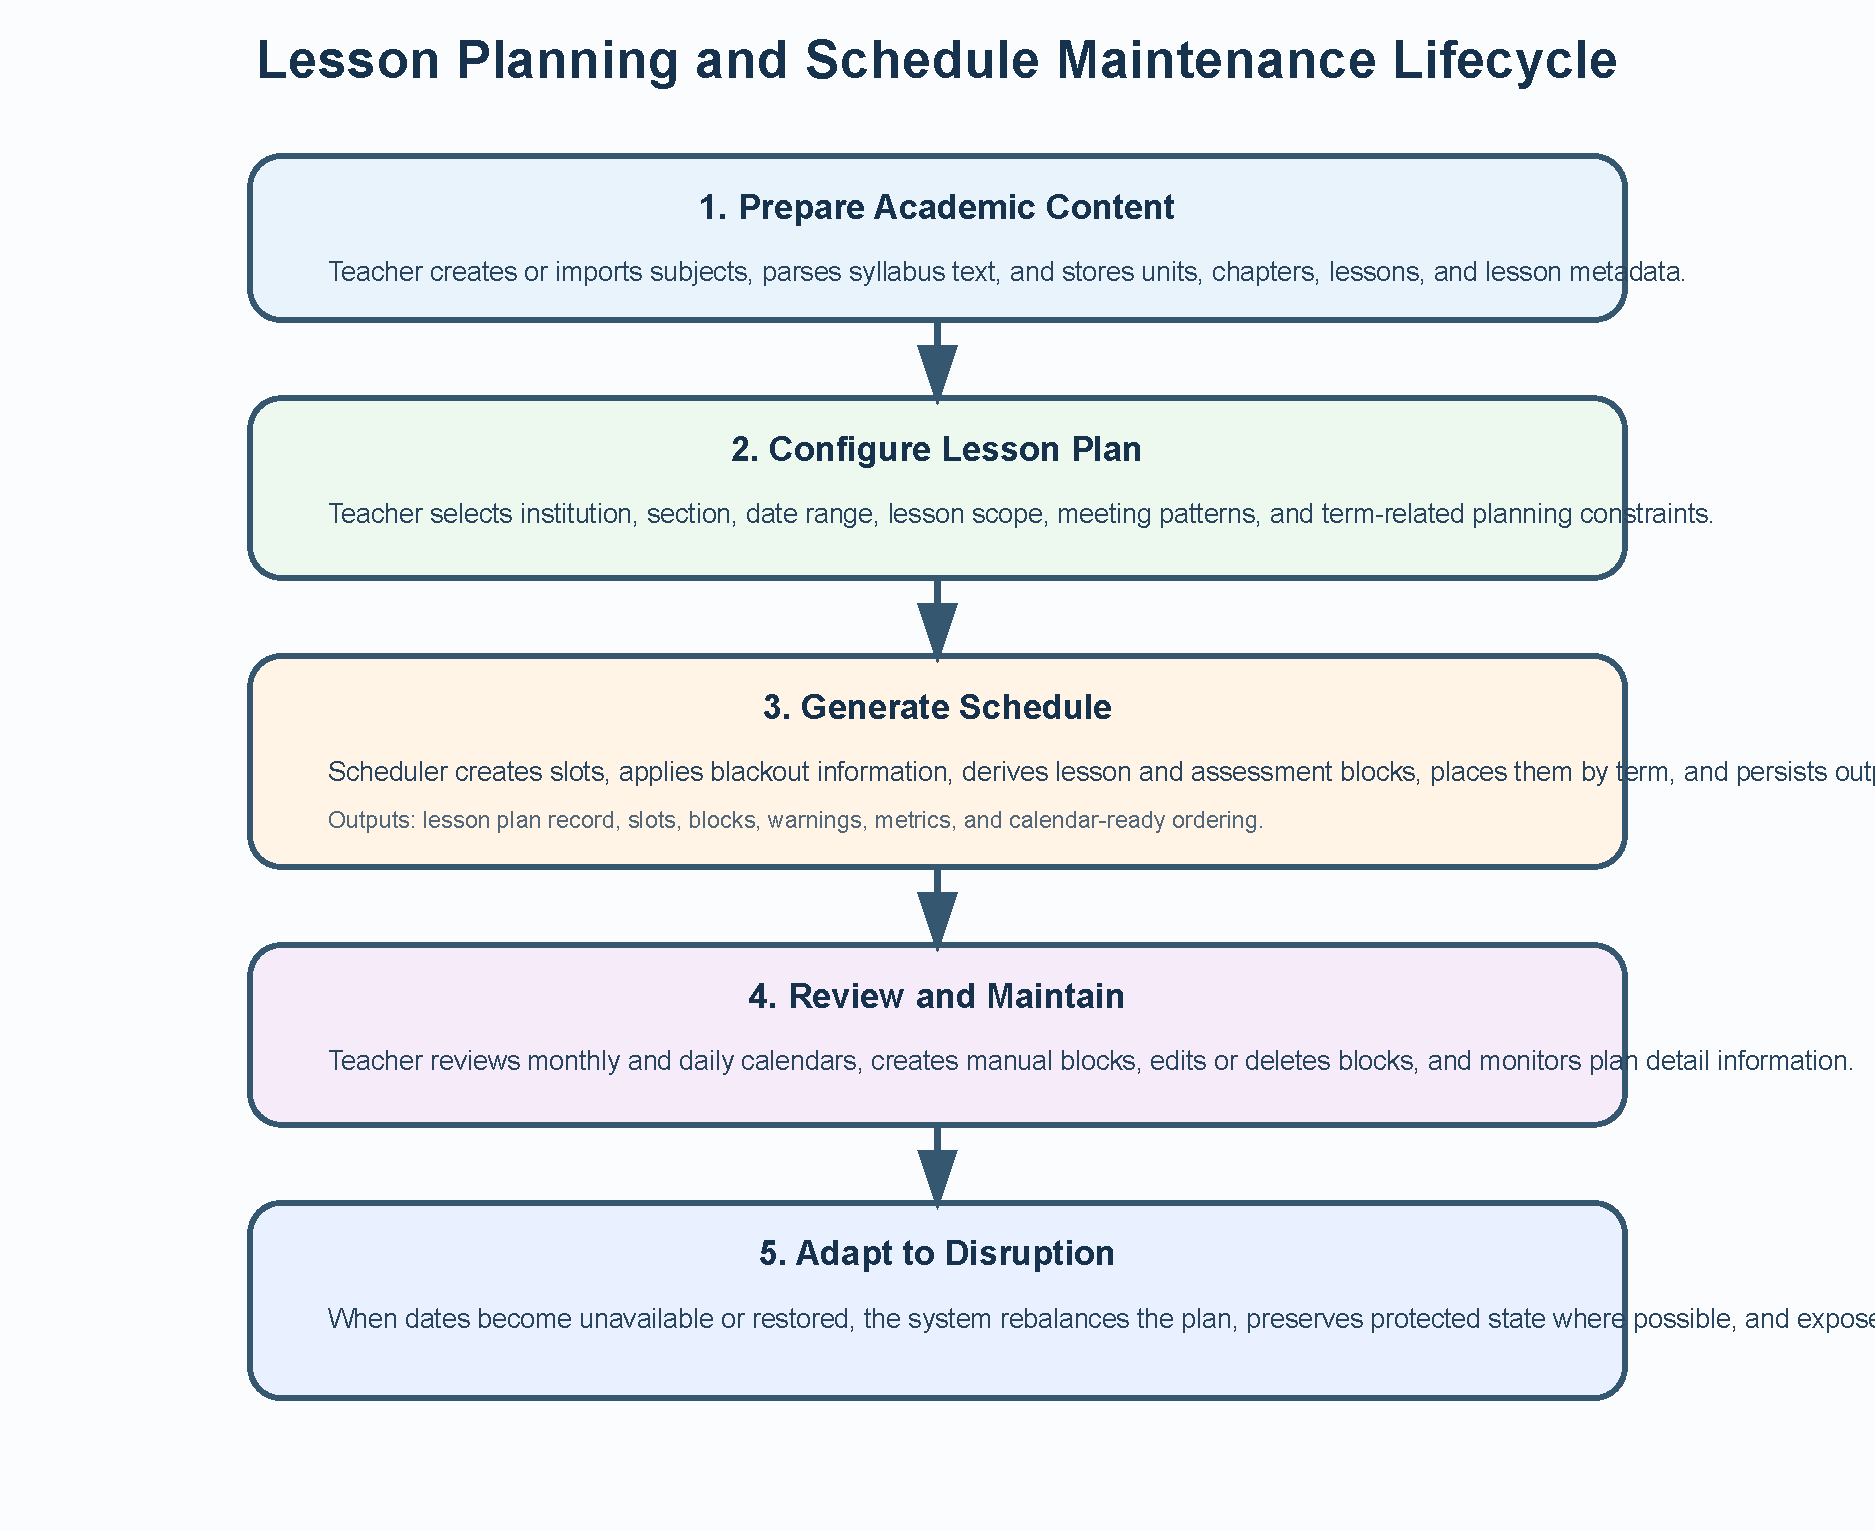
\includegraphics[height=0.28\textheight,keepaspectratio]{figures/scheduling-lifecycle.pdf}
\caption{Lesson planning and schedule maintenance lifecycle}
\label{fig:scheduling-lifecycle}
\end{figure}

\begin{longtable}{|L{2.3cm}|L{11.3cm}|}
\hline
\textbf{ID} & \textbf{Requirement} \\
\hline
FR-34 & The system shall allow a user to create a lesson plan for a selected institution, subject, and section. \\
\hline
FR-35 & The system shall require the user to define a lesson-plan start date and end date. \\
\hline
FR-36 & The system shall allow a user to define recurring meeting patterns including weekday, start time, end time, meeting type, and multiple class instances per day. \\
\hline
FR-37 & The system shall allow a user to define lesson-plan scheduling constraints, including academic term structure, special dates, blackout dates, and exam-related dates collected by the planner flow. \\
\hline
FR-38 & The system shall allow a user to select the lesson scope that will be included in the lesson plan. \\
\hline
FR-39 & The system shall allow a user to duplicate an existing lesson plan into a new draft. \\
\hline
FR-40 & The system shall validate lesson-plan input before generation or save. \\
\hline
FR-41 & The system shall generate schedule slots by expanding recurring meeting patterns into dated occurrences with slot numbers, series keys, and normalized time ranges. \\
\hline
FR-42 & The system shall apply blackout constraints from school calendar events and delays when generating or maintaining slots, and shall preserve compatible existing slot identifiers, lock flags, and manual state during regeneration. \\
\hline
FR-43 & The system shall partition the lesson plan into academic terms anchored by exam dates and shall derive lesson, quiz, written-work, performance-task, exam, and buffer blocks with term metadata and dependency information. \\
\hline
FR-44 & The system shall place generated blocks onto available slots using deterministic constraint-based greedy scheduling logic that reserves exam slots, assigns lesson blocks sequentially, and releases due assessments according to dependency and interval rules. \\
\hline
FR-45 & The system shall persist lesson-plan records, selected content scope, slots, and blocks after successful generation. \\
\hline
FR-46 & The system shall compute and expose schedule warnings and metrics for the generated plan, including total slots, usable slots, total blocks, placed blocks, unplaced blocks, category counts, and rebalance warnings. \\
\hline
FR-46A & The system shall rebalance a lesson plan deterministically after class-day availability changes by re-flowing non-locked blocks, preserving protected blocks, and surfacing locked-block conflicts instead of silently relocating teacher-pinned blocks. \\
\hline
FR-47 & The system shall allow a user to view lesson plans in a dedicated plans list. \\
\hline
FR-48 & The system shall allow a user to open a lesson-plan detail view showing metadata, status, and recurring schedule information. \\
\hline
FR-49 & The system shall allow a user to edit lesson-plan metadata and schedule-related draft details from the plan detail workflow. \\
\hline
\end{longtable}

\subsection{Calendar Viewing and Schedule Maintenance}

\textbf{Description:} This feature set presents generated schedules and supports
calendar-level maintenance operations.

\textbf{Priority: High}

\begin{longtable}{|L{2.3cm}|L{11.3cm}|}
\hline
\textbf{ID} & \textbf{Requirement} \\
\hline
FR-50 & The system shall display a monthly calendar view for a selected lesson plan. \\
\hline
FR-51 & The system shall allow the user to switch among available lesson plans in the calendar view. \\
\hline
FR-52 & The system shall display a daily agenda view containing scheduled blocks across the user's lesson plans for a selected date. \\
\hline
FR-53 & The system shall allow a user to select a day from the calendar and open its daily agenda. \\
\hline
FR-54 & The system shall allow a user to create a manual block for a selected day. \\
\hline
FR-55 & The system shall allow a user to edit an existing scheduled or manual block. \\
\hline
FR-56 & The system shall allow a user to delete a block from the daily agenda workflow. \\
\hline
FR-57 & The system shall allow a user to suspend or unsuspend selected lesson-plan entries from the daily agenda workflow using a recorded reason. \\
\hline
FR-58 & The system shall refresh plan and calendar screens after relevant planning or block-edit operations. \\
\hline
FR-59 & The system shall preserve teacher-locked or manually created schedule state during refresh and rebalance operations, unless the user explicitly edits or deletes that state. \\
\hline
FR-60 & The system shall allow a user to navigate from a daily agenda block to the related lesson, written-work, or performance-task detail when such detail exists. \\
\hline
\end{longtable}

\subsection{Activity Generation and Document Support}

\textbf{Description:} This feature set helps teachers create assessment documents
and supporting artifacts around planned instruction.

\textbf{Priority: Medium to High}

\begin{longtable}{|L{2.3cm}|L{11.3cm}|}
\hline
\textbf{ID} & \textbf{Requirement} \\
\hline
FR-61 & The system shall allow a user to create an activity draft under either the written-work or performance-task category. \\
\hline
FR-62 & The system shall allow a user to select an activity type appropriate to the selected category. \\
\hline
FR-63 & The system shall allow a user to select a subject and lesson scope for the activity. \\
\hline
FR-64 & The system shall allow a user to define activity requirements, selected components, and optional template guidance. \\
\hline
FR-65 & The system shall allow a user to upload template assets used to guide activity generation. \\
\hline
FR-66 & The system shall allow the user to invoke AI-assisted activity generation. \\
\hline
FR-67 & The system shall return generated activity text in an editable form. \\
\hline
FR-68 & The system shall allow the user to export generated activity output to PDF. \\
\hline
FR-69 & The system shall allow the user to export generated activity output to DOCX. \\
\hline
FR-70 & The system shall store generated activity metadata, selected scope, generated text, and artifact paths for later retrieval by the activity workflow. \\
\hline
FR-71 & The system shall provide curriculum text extraction support for uploaded subject or lesson source documents. \\
\hline
\end{longtable}

\subsection{Administrative Monitoring}

\textbf{Description:} This feature set provides an overview of current teachers,
plans, and planning progress for administrative users.

\textbf{Priority: Medium}

\begin{longtable}{|L{2.3cm}|L{11.3cm}|}
\hline
\textbf{ID} & \textbf{Requirement} \\
\hline
FR-72 & The system shall provide an administrative dashboard for authorized users. \\
\hline
FR-73 & The administrative dashboard shall display summary cards such as teacher count, subject count, lesson-plan count, and completion indicators from available backend records. \\
\hline
FR-74 & The administrative dashboard shall display current or upcoming lesson-plan information. \\
\hline
FR-75 & The administrative dashboard shall display teacher-related summaries such as names, roles, and plan counts from available backend records. \\
\hline
FR-76 & The administrative dashboard shall display recent planning or activity indicators derived from available backend records. \\
\hline
\end{longtable}

\section{Non-Functional Requirements}

\subsection{Performance Requirements}

\begin{longtable}{|L{2.3cm}|L{11.3cm}|}
\hline
\textbf{ID} & \textbf{Requirement} \\
\hline
NFR-01 & Under normal network conditions, the system should complete sign-in and initial route resolution within 5 seconds. \\
\hline
NFR-02 & Under normal network conditions, list screens such as plans and library should display primary content or a recoverable error state within 5 seconds after refresh is initiated. \\
\hline
NFR-03 & The system should complete schedule generation for a single lesson plan within 10 seconds for ordinary teacher planning workloads. \\
\hline
NFR-04 & Long-running extraction or generation tasks shall provide visible progress or status feedback to the user. \\
\hline
\end{longtable}

\subsection{Security and Privacy Requirements}

\begin{longtable}{|L{2.3cm}|L{11.3cm}|}
\hline
\textbf{ID} & \textbf{Requirement} \\
\hline
NFR-05 & The system shall use authenticated session management for protected features. \\
\hline
NFR-06 & The system shall restrict user-owned database and storage data through backend access controls such as RLS and authenticated storage rules. \\
\hline
NFR-07 & The system shall transmit client-backend traffic over HTTPS. \\
\hline
NFR-08 & The system shall isolate user file uploads by authenticated ownership path. \\
\hline
NFR-09 & The system shall be designed to support institutional privacy obligations, including proper handling of user account data and uploaded instructional documents. \\
\hline
\end{longtable}

\subsection{Reliability and Data Integrity Requirements}

\begin{longtable}{|L{2.3cm}|L{11.3cm}|}
\hline
\textbf{ID} & \textbf{Requirement} \\
\hline
NFR-10 & The system shall preserve lesson-plan, slot, and block records unless explicitly deleted by an authorized workflow. \\
\hline
NFR-11 & The system shall fail gracefully when backend or utility services are unavailable and shall provide an error message instead of silently discarding data. \\
\hline
NFR-12 & The scheduling pipeline shall behave deterministically for the same input state, producing the same slot, block, and ordering outcomes when the inputs remain unchanged. \\
\hline
NFR-13 & Rebalance operations shall preserve protected schedule state where the scheduler rules specify such behavior and shall behave idempotently for an unchanged schedule state. \\
\hline
\end{longtable}

\subsection{Usability Requirements}

\begin{longtable}{|L{2.3cm}|L{11.3cm}|}
\hline
\textbf{ID} & \textbf{Requirement} \\
\hline
NFR-14 & The application shall present mobile-friendly layouts suitable for handheld devices. \\
\hline
NFR-15 & The application shall provide understandable validation or error messages for failed form submissions and backend operations. \\
\hline
NFR-16 & The application shall support pull-to-refresh or equivalent refresh actions on major data views. \\
\hline
NFR-17 & The application shall support user-selectable appearance themes. \\
\hline
\end{longtable}

\subsection{Maintainability and Portability Requirements}

\begin{longtable}{|L{2.3cm}|L{11.3cm}|}
\hline
\textbf{ID} & \textbf{Requirement} \\
\hline
NFR-18 & The system shall maintain modular separation between UI flows, backend access helpers, and scheduling logic. \\
\hline
NFR-19 & The codebase shall remain TypeScript-based and lintable in the existing project toolchain. \\
\hline
NFR-20 & The primary production targets shall remain Android and iOS devices supported by the Expo/React Native stack. \\
\hline
NFR-21 & Utility features that require native capabilities shall degrade gracefully or document their runtime limitations. \\
\hline
NFR-22 & The defense build shall support a prepared live demonstration of authentication, academic setup, lesson-plan generation, calendar maintenance, and at least one document-support workflow. \\
\hline
NFR-23 & The project documentation shall distinguish implemented deterministic scheduling behavior from unsupported optimization claims. \\
\hline
\end{longtable}

\section{Acceptance Criteria and Traceability}

\subsection{Defense Acceptance Criteria}

The system shall be considered defense-ready when the following criteria are met:

\begin{longtable}{|L{2.7cm}|L{5.4cm}|L{5.4cm}|}
\hline
\textbf{ID} & \textbf{Acceptance Criterion} & \textbf{Verification Evidence} \\
\hline
AC-01 & A user can authenticate and reach protected teacher workflows. & Auth screens, protected route redirection, Supabase Auth session checks, and live sign-in demonstration. \\
\hline
AC-02 & A teacher can create or load institution, section, subject, chapter, and lesson data. & Profile, institution, library, subject-detail, lesson-detail, and lesson-editor screens backed by academic tables. \\
\hline
AC-03 & A teacher can create a lesson plan from selected subject content, date range, meeting patterns, and term settings. & Lesson-plan creation flow persists lesson plan, selected content, generated slots, and generated blocks. \\
\hline
AC-04 & The scheduler can generate a deterministic plan with placed lessons, assessments, exam anchors, metrics, and warnings. & Repository scheduler modules and passing \texttt{npm run test:scheduler} invariant execution. \\
\hline
AC-05 & A suspended or restored teaching day triggers deterministic rebalance without losing blocks. & Invariant harness covers suspend, unsuspend, compression, restoration, and idempotency scenarios. \\
\hline
AC-06 & A teacher-locked block that becomes infeasible is surfaced as a visible conflict rather than silently moved. & Invariant harness covers locked-block displacement, conflict warning, suggested re-pin slots, and re-pin recovery. \\
\hline
AC-07 & Calendar views display plan output and allow day-level inspection or maintenance. & Calendar monthly and daily screens, block editor workflow, refresh behavior, and live demo walkthrough. \\
\hline
AC-08 & Curriculum extraction and activity generation are guarded by authenticated backend calls. & Supabase Storage path ownership, \texttt{extract-text} Edge Function authentication, \texttt{generate-activity} validation, and prepared utility demo. \\
\hline
AC-09 & Administrative monitoring renders summary information for authorized users. & Admin route group and dashboard cards for teachers, subjects, plans, and recent activity. \\
\hline
AC-10 & Documentation and paper claims remain aligned with implementation boundaries. & This SRS, IEEE paper, scheduler invariant output, lint output, and explicit boundary section. \\
\hline
\end{longtable}

\subsection{Requirements Traceability Matrix}

\begin{longtable}{|L{2.5cm}|L{3.4cm}|L{4.2cm}|L{3.6cm}|}
\hline
\textbf{Req. Group} & \textbf{Implementation Area} & \textbf{Primary Data or Service} & \textbf{Validation Evidence} \\
\hline
FR-01--FR-09 & Authentication route group and root layout guards & Supabase Auth and user records & Live sign-in, sign-out, password recovery, route protection, and lint validation. \\
\hline
FR-10--FR-20 & Profile, settings, institution, and section screens & \texttt{users}, \texttt{schools}, \texttt{sections}, membership tables, storage avatars & Repository-backed workflow tracing and live profile/institution demo. \\
\hline
FR-21--FR-33 & Library, subject, lesson detail, and lesson editor screens & \texttt{subjects}, \texttt{units}, \texttt{chapters}, \texttt{lessons}, uploaded syllabus assets & Live subject/library demo and schema-backed persistence. \\
\hline
FR-34--FR-46A & Lesson-plan creation and scheduling engine & \texttt{lesson\_plans}, selected content, \texttt{slots}, \texttt{blocks}, scheduler modules & Passing scheduler invariants, generated metrics, and live lesson-plan generation. \\
\hline
FR-47--FR-60 & Plans list, plan detail, monthly calendar, daily agenda, block editor, and suspension actions & Persisted plan, slot, block, calendar event, and delay records & Live calendar walkthrough and rebalance invariant coverage. \\
\hline
FR-61--FR-71 & Activity creation, curriculum extraction, PDF/DOCX export, and sharing utilities & \texttt{activities}, Supabase Storage, \texttt{extract-text}, \texttt{generate-activity} & Edge Function guard inspection and prepared utility demo. \\
\hline
FR-72--FR-76 & Administrative route group and dashboard & User, subject, lesson-plan, activity, and completion summaries & Repository-backed admin screen tracing and authorized-role demo. \\
\hline
NFR-01--NFR-04 & App loading, refresh, scheduling, and long-running utility feedback & Expo runtime, Supabase network calls, scheduler pipeline & Live timing observation and visible loading/error states. \\
\hline
NFR-05--NFR-09 & Authentication, RLS, HTTPS, storage ownership, and privacy controls & Supabase Auth, PostgreSQL RLS, Storage policies, Edge Function bearer tokens & Schema and Edge Function inspection plus authenticated demo flow. \\
\hline
NFR-10--NFR-23 & Reliability, determinism, usability, maintainability, portability, demo readiness, and documentation accuracy & TypeScript modules, Expo screens, LaTeX documents, validation scripts & \texttt{npm run test:scheduler}, \texttt{npm run lint}, PDF rebuilds, and explicit limitations. \\
\hline
\end{longtable}

\subsection{Validation Status for Defense Package}

The current validation package is mixed but defensible for a live academic
defense. Scheduler behavior is directly validated by executable invariants. Code
style is checked by Expo linting, which currently reports no errors and known
warnings. Broader mobile workflows are validated by repository-backed tracing and
should be complemented with a live device walkthrough during defense. Utility
flows depend on configured Supabase functions and external service credentials,
so backup prepared records or screenshots should be available if the network or
AI service is unavailable during the presentation.

\section{Current System Boundaries}

The current version of SchEDU does \textbf{not} claim the following as supported
core features:
\begin{itemize}
\item institution-wide room allocation or campus-wide timetable optimization;
\item automated grading of student submissions;
\item full learning management system synchronization;
\item formal search-based optimization methods such as constraint programming or
simulated annealing; and
\item unrestricted offline operation for backend-dependent workflows.
\end{itemize}

These boundaries are intentional in this SRS so that the specification remains
aligned with the implemented repository and the current product scope.

\end{document}
